\section{Wie kann das AT in das ARFF-Format �berf�hrt werden?}\label{ATzuARFF}
Dazu wird ein Programm in Java namens Text2ARFFConverter entwickelt. Es liest alle W�rter die im AT vorkommen ein, filtert doppelte dabei aus. Dann z�hlt es, wie h�ufig die W�rter im AT vorkommen. Es sortiert dann die W�rter nach H�ufigkeit. Mit einem Startparameter kann angegeben werden, wie viele W�rte bzw. Attribute in den Header der zu erzeugenden ARFF-Datei geschreiben werden sollen. Wird das Programm mit 100 gestartet, werden bei der Erzeugung der ARFF-Datei die 100 am h�ufigsten vorkommenden W�rter als Attribute in die ARFF geschrieben. Im Datenteil der ARFF-Datei werden die Instanzen erzeugt. Dazu wird das AT Zeilenweise eingelesen. Wenn sich ein Wort unter den z.B. h�ufigsten 100 W�rtern befindet, wird gez�hlt wie oft es im Satz vorkommt. Wurden alle W�rter eines Verses gez�hlt, kann die Instanz geschrieben werden.

\section{Analyse Text2ARFFConverter}\label{AnalyseText2ARFFConverter}

In Abbildung \ref{fig:Analyseklassendiagramm_Text2ARFFConverter} auf Seite \pageref{fig:Analyseklassendiagramm_Text2ARFFConverter} ist das Analyseklassendiagramm des Text2ARFF\-Con\-ver\-ters zu sehen.

\begin{figure}[htp]
\centering
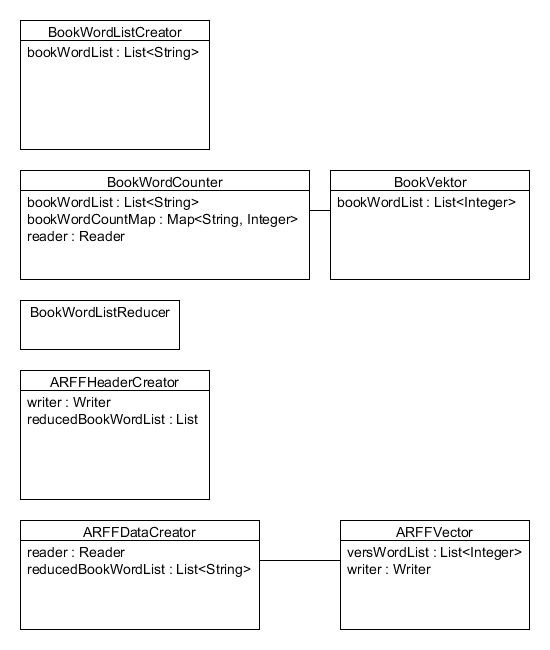
\includegraphics[width=1\textwidth]{Ingo/Bilder/Analyseklassendiagramm_Text2ARFFConverter.png}
\caption{Analyseklassendiagramm Text2ARFFConverter}
\label{fig:Analyseklassendiagramm_Text2ARFFConverter}
\end{figure}

\section{Entwurf Text2ARFFConverter}\label{EntwurfText2ARFFConverter}

In Abbildung \ref{fig:Entwurfsklassendiagramm_Text2ARFFConverter} auf Seite \pageref{fig:Entwurfsklassendiagramm_Text2ARFFConverter} ist das Entwurfsklassendiagramm des Text2ARFF\-Con\-ver\-ters zu sehen.

\begin{figure}[htp]
\centering
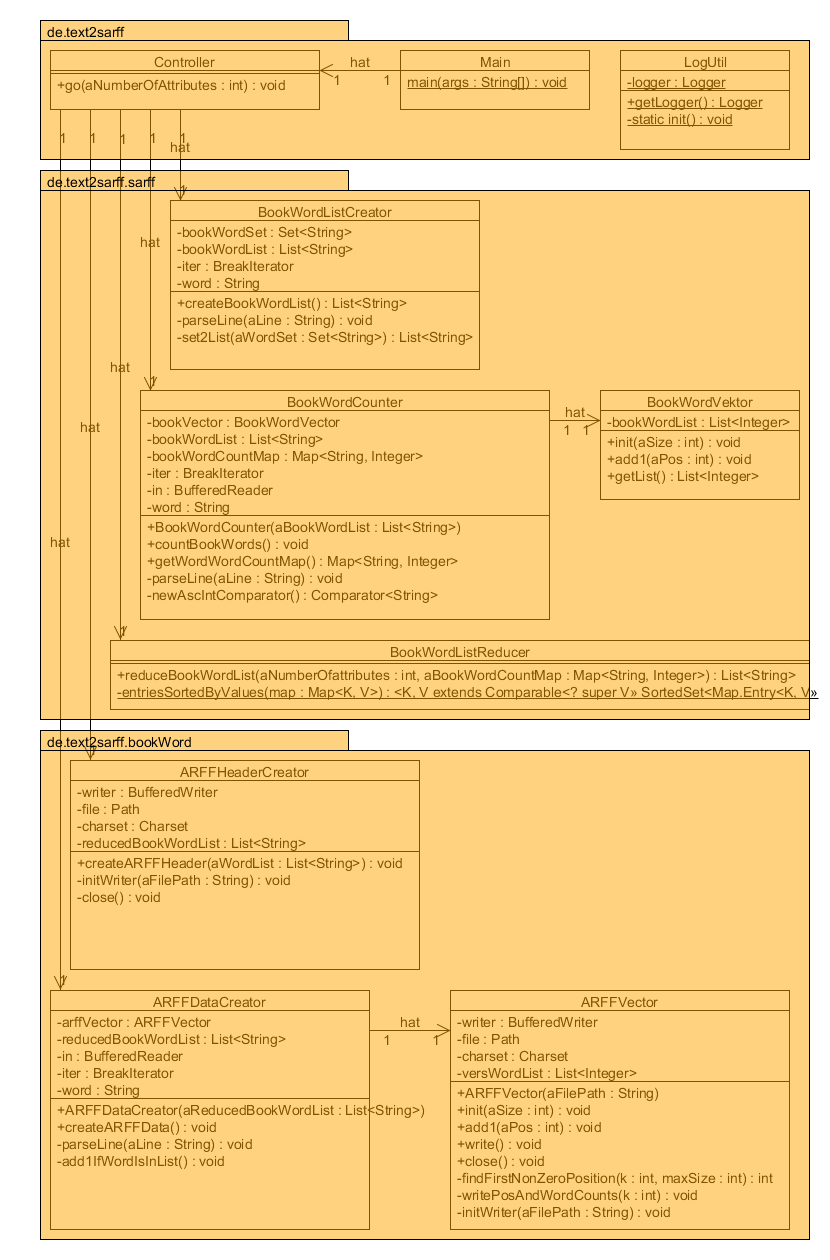
\includegraphics[width=1\textwidth]{Ingo/Bilder/Entwurfsklassendiagramm_Text2ARFFConverter.png}
\caption{Entwurfsklassendiagramm Text2ARFFConverter}
\label{fig:Entwurfsklassendiagramm_Text2ARFFConverter}
\end{figure}

\cite{bib1} \cite{bib2}